\documentclass[11pt]{article}

% ---------- Typography: clean, professional, journal-style ----------
\usepackage[T1]{fontenc}
\usepackage[utf8]{inputenc}
\usepackage{amsmath,amssymb,amsthm}   % load before newtxmath to avoid \Bbbk clash
\usepackage{newtxtext,newtxmath}     % Times-like serif, professional look
\usepackage[margin=1in]{geometry}
\usepackage{microtype}                % subtle spacing/kerning polish
\usepackage{setspace}
\setstretch{1.05}

% ---------- Structure & references ----------
\usepackage{booktabs}                 % clean table rules, no vertical lines
\usepackage{caption}
\usepackage{subcaption}
\usepackage{graphicx}
\usepackage[colorlinks=true,citecolor=blue!55!black,linkcolor=blue!55!black,urlcolor=blue!55!black]{hyperref}
\usepackage[round,authoryear]{natbib}
\usepackage{xcolor}
\usepackage{enumitem}
\setlist{topsep=4pt,itemsep=2pt}
\usepackage{tikz}
\usetikzlibrary{positioning,fit,arrows.meta,calc,decorations.pathreplacing}
\definecolor{v2blue}{RGB}{0,114,178}
\definecolor{twinverm}{RGB}{213,94,0}

% ---------- Section spacing (tight, professional) ----------
\usepackage{titlesec}
\titlespacing*{\section}{0pt}{14pt}{6pt}
\titlespacing*{\subsection}{0pt}{10pt}{4pt}

% ---------- Draft-status callouts (visible in compiled PDF, remove before submission) ----------
\newcommand{\blocked}[1]{%
  \par\smallskip
  \noindent\fcolorbox{orange!70!black}{orange!8}{%
    \begin{minipage}{0.96\linewidth}
    \small\color{orange!40!black}\textbf{[BLOCKED --- draft placeholder]} #1
    \end{minipage}%
  }
  \smallskip\par
}
\newcommand{\readynote}[1]{%
  {\small\color{gray}\textit{#1}}
}

\title{\textbf{When Does Generative Forecasting Pay Off? \\
  \large A Controlled Deterministic--Diffusion Comparison for \\
  Flood Prediction under Sparse Observation}}
\author{Wissam Abdelwahed}
\date{\today}

\begin{document}
\maketitle

\begin{abstract}
\noindent
Conditional diffusion models are increasingly applied to spatiotemporal
forecasting under partial observation, on the premise that a generative
model's sampling distribution provides value a deterministic model cannot.
We test this premise directly for autoregressive flood forecasting on
FloodCastBench, using a \emph{parameter- and protocol-matched deterministic
twin} of our diffusion model as a controlled baseline --- to our knowledge
the first such matched control for this task. We first identify and correct
a structural failure mode of diffusing the \emph{absolute} water-depth
field at fine temporal resolution (a sampling-noise floor exceeding the
true physical signal by a factor of $\sim\!450$--$490\times$, measured
directly on two independent flood events), motivating a delta-space,
per-regime-scaled parametrization. The corrected model then outperforms
the published FNO+ operator baseline on all reported metrics in the fully
observed regime. Against its own deterministic twin, however, the
generative model's advantage is not uniform: \blocked{final verdict pending
re-evaluation on corrected checkpoints --- see \S\ref{sec:results}.} We
further evaluate calibration under partial observation, generalization to
structured (non-i.i.d.) sensor layouts, and \blocked{cross-event transfer
and a deep-ensemble uncertainty baseline (in progress).} We report this
comparison in full, including where it does not favor the generative
approach, as we believe controlled negative results of this kind are
currently underrepresented in this literature.
\end{abstract}

\begin{center}
\readynote{Draft compiled \today\ --- sections marked BLOCKED depend on in-progress experiments;\\ see \texttt{reports/paper\_master\_plan.md} for live status.}
\end{center}

% ============================================================
\section{Introduction}
\label{sec:intro}
\blocked{Written last, once the full results are frozen. Structural notes: (1) motivate the deployment scenario --- sparse sensor networks, why full-field observation is unrealistic; (2) state the central question, ``when is a generative model's extra machinery justified over a matched deterministic model?''; (3) list contributions in order of strength --- the matched-twin control itself, the quantified failure mechanism (\S\ref{sec:mechanism}), the reinstated causal input (Manning roughness from LULC, \S\ref{sec:manning} if completed), and the reusable evaluation protocol (multi-seed, oracle+sparse persistence, calibration).}

% ============================================================
\section{Related Work}
\label{sec:related}

Diffusion-based reconstruction under sparse observation has been explored
along two largely disjoint lines. The first targets tidal and coastal
flood forecasting directly: \citet{diffsparse2025} diffuse a coastal
water-level field under 0/50/95\% sparsity and report up to 62\% error
reduction over baseline methods, but do not include a parameter-matched
deterministic control, do not diagnose a failure mechanism for their own
parametrization, and do not evaluate the calibration of their generated
ensembles. \citet{spatiallyawarediffusion2024} reconstruct static PDE
fields from sparse sensors with a hybrid conditioning scheme close to our
spatial encoder, and --- notably --- independently conclude that a
deterministic model wins in the noise-free regime while diffusion only
helps once observation noise is introduced; we extend this finding to the
\emph{autoregressive}, real-benchmark setting and quantify a concrete
parametrization-level mechanism for it (\S\ref{sec:mechanism}). A second
line applies conditional diffusion to data assimilation at
national-to-global scale for weather and ocean state
\citep{jamesstations2025,jamesocean2025,phyda2025} --- an active area, but
none of this work runs a matched deterministic control, and none targets
pluvial or fluvial flood forecasting. \citet{sf2bench2025} provide real
river-gauge time series but no spatial field reconstruction, making it
complementary rather than substitutable. \citet{floodcastbench2025} is, to
our knowledge, the only public benchmark combining high-fidelity flood
fields, physical forcings (DEM, rainfall), and neural-operator baselines
(U-Net, FNO, FNO+) at the resolution and cadence used here, and is the
benchmark we build on.

No existing work, to our knowledge, runs a parameter- and protocol-matched
deterministic-vs-generative comparison for autoregressive flood forecasting
under sparse observation. This is the gap we address.

% ============================================================
\section{Problem Setup}
\label{sec:setup}

\subsection{Task}
We consider the task of forecasting the spatiotemporal evolution of a
flood --- a dense field of water depth over a fixed spatial grid --- from a
\emph{partially observed} current state. At full observation density
(``dense''), the current water-depth field is known everywhere; under
sparsity, only a subset of grid cells (a proxy for a real sensor network)
is observed at each time step, with the rest masked. The forecasting
horizon is autoregressive: models roll forward multiple 300-second steps,
re-consuming their own (or the sparsely-observed) state at each step.

\subsection{Benchmark}
We use FloodCastBench's high-fidelity Australia event at 60\,m resolution
\citep{floodcastbench2025}: 2{,}881 water-depth frames at 300\,s cadence
($536\times536$ grid), paired with a static digital elevation model (DEM)
and time-varying rainfall forcing at 1800\,s resolution (repeated across
the six 300\,s frames each covers, matching the official data-generation
convention). \blocked{Report a second event (UK, 2015) here once WP8/WP10 complete --- see \S\ref{sec:limitations} for current status.}

\subsection{Sparsity protocol}
We evaluate three observation regimes: dense (100\% observed), \textsc{m50}
(50\% missing), and \textsc{m95} (95\% missing) --- a random i.i.d.\ mask
sampled per evaluation window from a fixed bank of 10 masks (seeded, reused
across models for a fair comparison). To test whether conclusions drawn
under random masking generalize to \emph{realistic} sensor deployments, we
additionally evaluate two structured mask families never seen during
training: a \textbf{gauge} proxy (sensors weighted toward high initial
water-occupancy cells, approximating river-gauge placement) and a
\textbf{cluster} mask (spatially contiguous unobserved regions,
approximating a coverage gap) --- \S\ref{sec:masks}.

\subsection{What ``calibration'' can mean here}
FloodCastBench's ground truth is generated by a single deterministic
hydraulic simulation (Saint-Venant) per event --- there is no ensemble of
physical realizations to calibrate against. The uncertainty a generative
model's scenario spread can meaningfully quantify here is therefore the
\emph{ambiguity of reconstruction under partial observation} (how many
distinct complete fields are consistent with a given sparse observation),
not aleatoric physical uncertainty. We evaluate calibration under this
reading throughout, and state it explicitly rather than let the term imply
more than the data can support.

% ============================================================
\section{Methods}
\label{sec:methods}

\subsection{The controlled pair: a diffusion model and its deterministic twin}
\label{sec:twin}
To isolate whether a generative model's value comes from its generative
mechanism specifically --- as opposed to its architecture, training
budget, or context length --- we construct a \textbf{deterministic twin}: a
model sharing our diffusion model's (``V2'') exact encoders (temporal
context encoder, pixel-aligned spatial encoder), backbone (2D U-Net),
parameter count (verified by direct comparison, not approximate), training
budget, checkpoint-selection protocol, and pushforward scheme, with the
diffusion loop replaced by a single deterministic forward pass (noise
input fixed to zero, no diffusion timestep). This is, to our knowledge, the
first such matched control run for autoregressive flood forecasting under
sparsity. Figure~\ref{fig:pair} summarizes the shared architecture and the
single point at which the two models differ.

\begin{figure}[t]
\centering
\resizebox{\linewidth}{!}{%
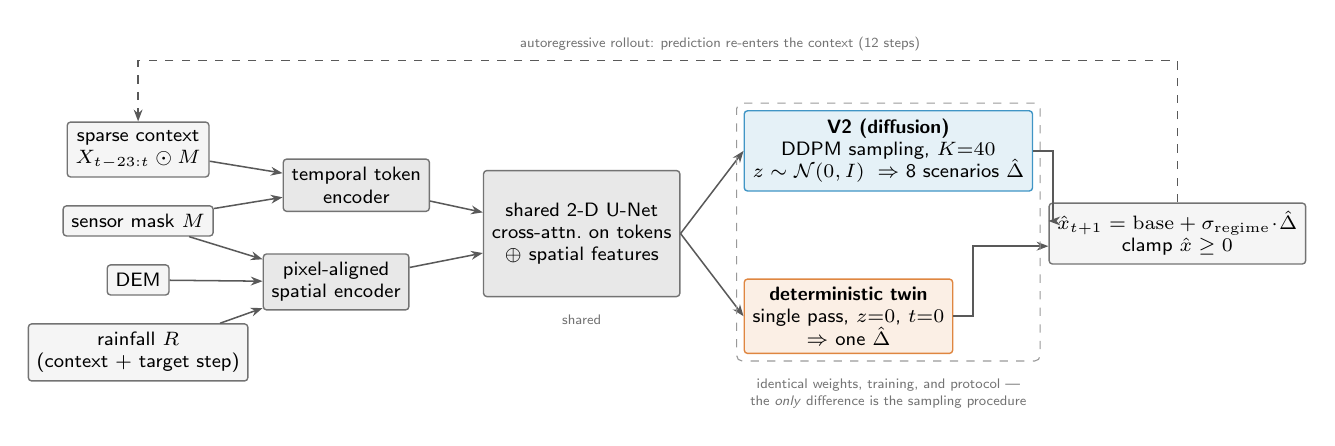
\begin{tikzpicture}[
  font=\sffamily\scriptsize,
  node distance=3.5mm and 6mm,
  box/.style={draw=black!55, rounded corners=1.2pt, align=center, inner sep=3pt, fill=black!4, line width=0.5pt},
  enc/.style={box, fill=black!9},
  headv/.style={box, fill=v2blue!10, draw=v2blue!75},
  headt/.style={box, fill=twinverm!10, draw=twinverm!75},
  arr/.style={-{Stealth[length=1.5mm]}, black!65, line width=0.55pt},
  lab/.style={font=\sffamily\tiny, black!55, align=center},
]
% ---- inputs ----
\node[box] (xin) {sparse context\\ $X_{t-23:t}\odot M$};
\node[box, below=of xin] (min) {sensor mask $M$};
\node[box, below=of min] (dem) {DEM};
\node[box, below=of dem] (rain) {rainfall $R$\\ (context $+$ target step)};
% ---- shared encoders ----
\node[enc, right=9mm of $(xin.east)!0.5!(min.east)$] (tenc) {temporal token\\ encoder};
\node[enc, right=9mm of $(dem.east)!0.5!(min.east)$, yshift=-4mm] (senc) {pixel-aligned\\ spatial encoder};
% ---- shared U-Net ----
\node[enc, right=8mm of $(tenc.east)!0.5!(senc.east)$, minimum height=16mm] (unet) {shared 2-D U-Net\\ cross-attn.\ on tokens\\ $\oplus$ spatial features};
% ---- two inference heads ----
\node[headv, anchor=west] (v2) at ($(unet.east)+(8mm,10.5mm)$) {\textbf{V2 (diffusion)}\\ DDPM sampling, $K{=}40$\\ $z\sim\mathcal N(0,I)\;\Rightarrow\;$8 scenarios $\hat\Delta$};
\node[headt, anchor=west] (tw) at ($(unet.east)+(8mm,-10.5mm)$) {\textbf{deterministic twin}\\ single pass, $z{=}0$, $t{=}0$\\ $\Rightarrow$ one $\hat\Delta$};
% ---- reconstruction ----
\node[box, right=7mm of $(v2.east)!0.5!(tw.east)$] (rec) {$\hat x_{t+1}=\mathrm{base}+\sigma_{\mathrm{regime}}\!\cdot\!\hat\Delta$\\ clamp $\hat x\ge 0$};
% ---- arrows ----
\draw[arr] (xin) -- (tenc);
\draw[arr] (min) -- (tenc);
\draw[arr] (min) -- (senc);
\draw[arr] (dem) -- (senc);
\draw[arr] (rain) -- (senc);
\draw[arr] (tenc) -- (unet);
\draw[arr] (senc) -- (unet);
\draw[arr] (unet.east) -- (v2.west);
\draw[arr] (unet.east) -- (tw.west);
\draw[arr] (v2.east) -- ++(2.5mm,0) |- ($(rec.west)+(0,1.6mm)$);
\draw[arr] (tw.east) -- ++(2.5mm,0) |- ($(rec.west)+(0,-1.6mm)$);
% autoregressive feedback
\draw[arr, dashed] (rec.north) -- ++(0,18mm) -| node[pos=0.22, above, lab] {autoregressive rollout: prediction re-enters the context (12 steps)} (xin.north);
% shared-vs-differs annotation
\node[draw=black!40, dashed, rounded corners=2pt, fit=(v2)(tw), inner sep=2.5pt] (differ) {};
\node[lab, below=1mm of differ.south] {identical weights, training, and protocol --- \\ the \emph{only} difference is the sampling procedure};
\node[lab, below=1mm of unet.south] {shared};
\end{tikzpicture}%
}
\caption{The controlled pair. Both models share every component --- inputs,
temporal token encoder, pixel-aligned spatial encoder, U-Net backbone,
delta-space target with per-regime scale $\sigma_{\mathrm{regime}}$
(\S\ref{sec:mechanism}), training protocol, and autoregressive rollout.
The diffusion model (V2) samples $K{=}40$ denoising steps from Gaussian
noise to produce 8 scenarios; the twin evaluates the same network once with
$z{=}0$, $t{=}0$. Any performance difference is therefore attributable to
the generative mechanism itself.}
\label{fig:pair}
\end{figure}

\paragraph{A statistical trap in comparing the two, and why it matters.}
For any posterior distribution,
\begin{equation}
\mathbb{E}\big[(x_{\text{sample}} - x_{\text{truth}})^2\big]
  = \mathrm{Var}(\text{posterior}) + \mathbb{E}\big[(\bar{x} - x_{\text{truth}})^2\big]
  \;\geq\; \mathbb{E}\big[(\bar{x} - x_{\text{truth}})^2\big],
\end{equation}
so a single draw from a generative model carries strictly more expected
squared error than the posterior mean, purely as a property of variance,
regardless of model quality. A deterministic regressor targets the mean
directly. Comparing a single generative draw to a deterministic output on
RMSE is therefore \textbf{mathematically biased toward the deterministic
model by construction} --- we discovered this affecting our own internal
checkpoint-selection metric mid-project (it uses a single rollout draw) and
correct for it by reporting only twin-vs-\emph{mean-of-8-scenarios}
comparisons as decision-relevant throughout this paper. We flag this
explicitly as a generic trap for any future deterministic-vs-generative
comparison in this literature.

\subsection{Why the field's absolute value cannot be diffused directly at fine cadence}
\label{sec:mechanism}
A first attempt (``V1'', following the reference parametrization of
\citealp{diffsparse2025}) diffusing the \emph{absolute} water-depth field
at the benchmark's native 300-second cadence fails catastrophically in the
dense regime: $\sim\!560\times$ worse than trivial persistence (predicting
no change). We trace this to a scale mismatch, not an implementation
defect: the true physical signal between two 300-second frames
($\sigma_\Delta$, the frame-to-frame standard deviation) is tiny relative
to the field's own scale ($\sigma_{\text{field}}$) --- we measure the ratio
at
\begin{equation}
\sigma_{\text{field}} / \sigma_\Delta \;\approx\; 488 \text{ (Australia)}, \quad 425 \text{ (UK)}
\end{equation}
across both tested events (Figure~\ref{fig:mechanism}). A diffusion
sampler's own residual error scales with the magnitude of \emph{its
generative target}; diffusing the absolute field makes that target the
full field scale, so beating persistence requires a per-step sampling
error under $\sim\!0.2\%$ of the field's own range --- below what a
realistic diffusion sampler achieves at this resolution. Our model
(``V2'') instead diffuses the \emph{delta} (the frame-to-frame change),
for which the equivalent condition is trivially satisfied.

\begin{figure}[t]
  \centering
  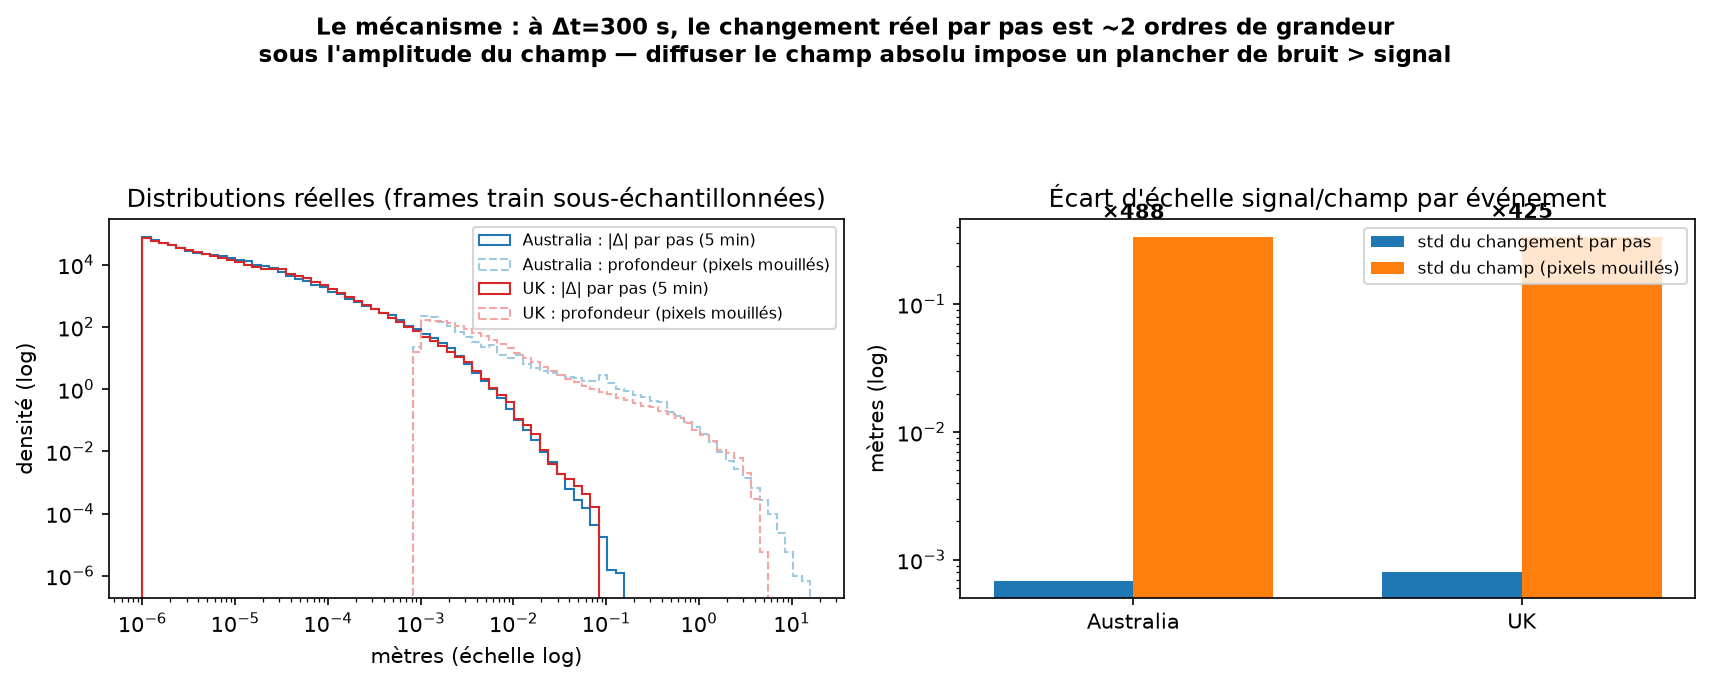
\includegraphics[width=0.92\linewidth]{figures/f2_mechanism.png}
  \caption{The sampling-noise floor mechanism: distribution of frame-to-frame
  deltas versus the absolute field, measured directly from training data,
  for both tested events. The field-to-delta scale ratio ($\sim\!488\times$
  Australia, $\sim\!425\times$ UK) sets a lower bound on the per-step
  sampling accuracy a diffusion model must achieve to beat trivial
  persistence when diffusing the absolute field.}
  \label{fig:mechanism}
\end{figure}

\subsection{Per-regime scale under partial observation}
Under sparsity, a further complication arises: an observed pixel's natural
target scale is the delta from its last known value ($\sigma_\Delta$); a
masked pixel's target is the delta from the training-mean fill, whose scale
is closer to $\sigma_{\text{field}}$. A single global scale for both
regimes either drowns the observed-pixel signal or destabilizes the
masked-pixel one --- an instability we encountered directly during
development (NaN batches under exactly this defect, corrected and
regression-tested). V2 therefore uses a \textbf{per-pixel, regime-aware
scale}, resolved at each pixel from its observed/masked status at the
current step.

\subsection{Architecture summary}
V1 uses the reference DIFF-SPARSE architecture at context length 12; V2
widens the temporal token encoder, adds a pixel-aligned spatial context
pathway, and extends the context length to 24. This context extension is
itself ablated: a context-length-12 V2 (matched to V1) still dominates V1
by $970\times$ (dense), $3.9\times$ (\textsc{m50}), $1.9\times$
(\textsc{m95}) on a seed-42 screening evaluation \blocked{confirm at 3 seeds before freezing --- currently single-seed} --- the architectural gain is not merely a longer-context artifact.

% ============================================================
\section{Evaluation Protocol}
\label{sec:protocol}
\blocked{Full protocol paragraph: test split window count (13/13 at native
protocol), \texttt{tile\_stride}, patch size, blending, number of
evaluation scenarios (2 val / 8 test), fixed mask bank, oracle- and
sparse-persistence both reported, multi-seed reporting convention (mean
$\pm$ std, $N$ stated), significance testing to add before freezing
(paired bootstrap or signed-rank across the 13 test windows $\times$ 3
seeds) --- port directly from \texttt{paper\_master\_plan.md} \S5.}

% ============================================================
\section{Results}
\label{sec:results}

\subsection{V2 vs.\ the published FNO+ result, all metrics}
\label{sec:vsfnoplus}
A natural objection to any ``V2 beats FNO+'' claim is that it might simply
reflect an imperfect FNO+ reproduction (our own reproduction sits
$1.66\times$ above the published Table~4 relative RMSE, a gap traced to
undisclosed preprocessing details, not a bug). We therefore also report V2
against the \emph{published} number directly, sidestepping that objection
entirely (Table~\ref{tab:vsfnoplus}).

\begin{table}[t]
\centering
\caption{V2 (dense, mean $\pm$ std over 3 seeds) versus the \emph{published}
FNO+ Table~4 result. V2 outperforms on all five reported metrics.
\blocked{quick 4/13-window read --- rerun at full 13/13 before freezing.}}
\label{tab:vsfnoplus}
\begin{tabular}{lrr}
\toprule
Metric & FNO+ (published) & V2 dense (ours) \\
\midrule
Relative RMSE $\downarrow$ & 0.003941 & $0.001576 \pm 0.000818$ \\
NSE $\uparrow$              & 0.999979 & $0.999996 \pm 0.000004$ \\
Pearson $r$ $\uparrow$      & 0.999990 & $0.999999 \pm 0.000001$ \\
CSI@0.001 $\uparrow$        & 0.939638 & $0.986660 \pm 0.003735$ \\
CSI@0.01 $\uparrow$         & 0.984588 & $0.999098 \pm 0.000393$ \\
\bottomrule
\end{tabular}
\end{table}

This holds even though V2's input context (24 frames) exceeds FNO+'s
(1 frame --- the official architecture's ``20-frame'' input tensor
broadcasts one observed value across all time positions, not a real
temporal signal) --- a natural objection we tested directly rather than
dismissed: giving FNO+ the \emph{same} 24-frame context makes it
\textbf{worse}, not better (relative RMSE $0.007529\pm0.000328$ vs.\ its
own $0.006550\pm0.000135$ baseline, confirmed at 3 seeds), so extra context
alone does not explain V2's margin.

\subsection{Parametrization dominates; context length does not explain it}
\label{sec:paramresults}
Figure~\ref{fig:sparsity} compares the four members of the model family
across observation regimes. Two facts stand out. First, the delta-space
parametrization is worth up to three orders of magnitude: V1 sits at or
above the persistence level everywhere (its dense-regime error is
$\sim$560$\times$ persistence), while every delta-space model is far below
it. Second, this is not a context-length artifact: a V2 retrained at V1's
own context length (12 frames) retains essentially the entire advantage
(dense $970\times$, \textsc{m50} $3.9\times$, \textsc{m95} $1.9\times$ over
V1 on the screening evaluation) --- consistent with \S\ref{sec:vsfnoplus},
where \emph{giving} the baseline more context made it worse.

\begin{figure}[t]
  \centering
  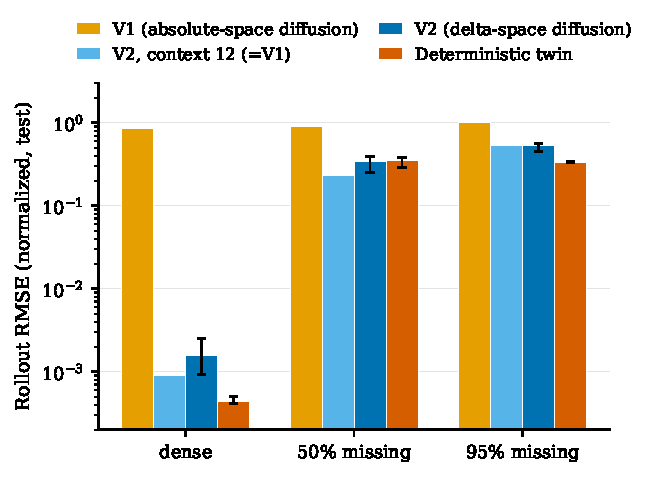
\includegraphics[width=0.78\linewidth]{figures/f3_performance_sparsity.pdf}
  \caption{Rollout RMSE (normalized, test) across observation regimes,
  log scale. V1/V2-ctx12: seed 42 screening read; V2 and twin: mean of
  3 seeds, error bars span the seed range. \emph{Sparse-regime V2/twin
  values are preliminary}: a convergence audit (\S\ref{sec:protocol})
  found the original sparse checkpoints under-trained, and the corrected
  re-evaluation was in progress at the time of writing.}
  \label{fig:sparsity}
\end{figure}

\subsection{Deterministic twin vs.\ V2: the central comparison}
\label{sec:twinresults}
\blocked{THE headline table (Table~T2 in the working plan). Currently being
re-evaluated: an extended-training-budget audit found the sparse-regime
checkpoints (both V2 and the twin) were systematically under-converged in
the original runs ($-16\%$ to $-37\%$ improvement in the internal
checkpoint-selection metric after retraining with a longer budget and
patience --- one run never converged even at 600 epochs). Both families are
being retrained/re-evaluated on the corrected checkpoints before this table
is frozen. Pre-registered decision criteria (unchanged): twin
$\geq$ V2-mean-of-8-scenarios everywhere $\Rightarrow$ thesis fails, write
it as such; V2 wins in sparse and ties/loses in dense $\Rightarrow$ thesis
confirmed; mixed $\Rightarrow$ report by regime, no blanket claim.}

\subsection{Structured masks vs.\ random}
\label{sec:masks}
Training uses i.i.d.\ random observation masks; deployment sensor networks
are not i.i.d. We test two structured mask families never seen in
training, at matched sensor budget (Table~\ref{tab:masks}).

\begin{table}[t]
\centering
\caption{V2 relative RMSE under structured vs.\ random masks (seed 42;
cluster/\textsc{m50} confirmed on a second seed, relative RMSE 0.597 vs.\
0.609).}
\label{tab:masks}
\begin{tabular}{lrrl}
\toprule
Mask & \textsc{m50} & \textsc{m95} & vs.\ random \\
\midrule
Random (training distribution) & 0.395 & 0.567 & --- \\
Gauge (spatially distributed)  & 0.393 & 0.585 & $\approx$ identical \\
Cluster (contiguous gap)       & 0.609 & 0.706 & \textbf{+54\% / +25\%} \\
\bottomrule
\end{tabular}
\end{table}

The \textbf{gauge} mask --- despite being structured rather than i.i.d.\ ---
remains spatially distributed, and the model generalizes to it almost
perfectly. The \textbf{cluster} mask leaves a large contiguous region
entirely unobserved, a spatial regime never encountered during training,
and degrades markedly. This is a real, physically interpretable
generalization boundary: the model's implicit assumption is
\emph{distributed} partial observation, not merely a sensor \emph{count}
--- worth stating plainly as a deployment limitation.

\subsection{Calibration}
\label{sec:calibration}
\begin{figure}[t]
  \centering
  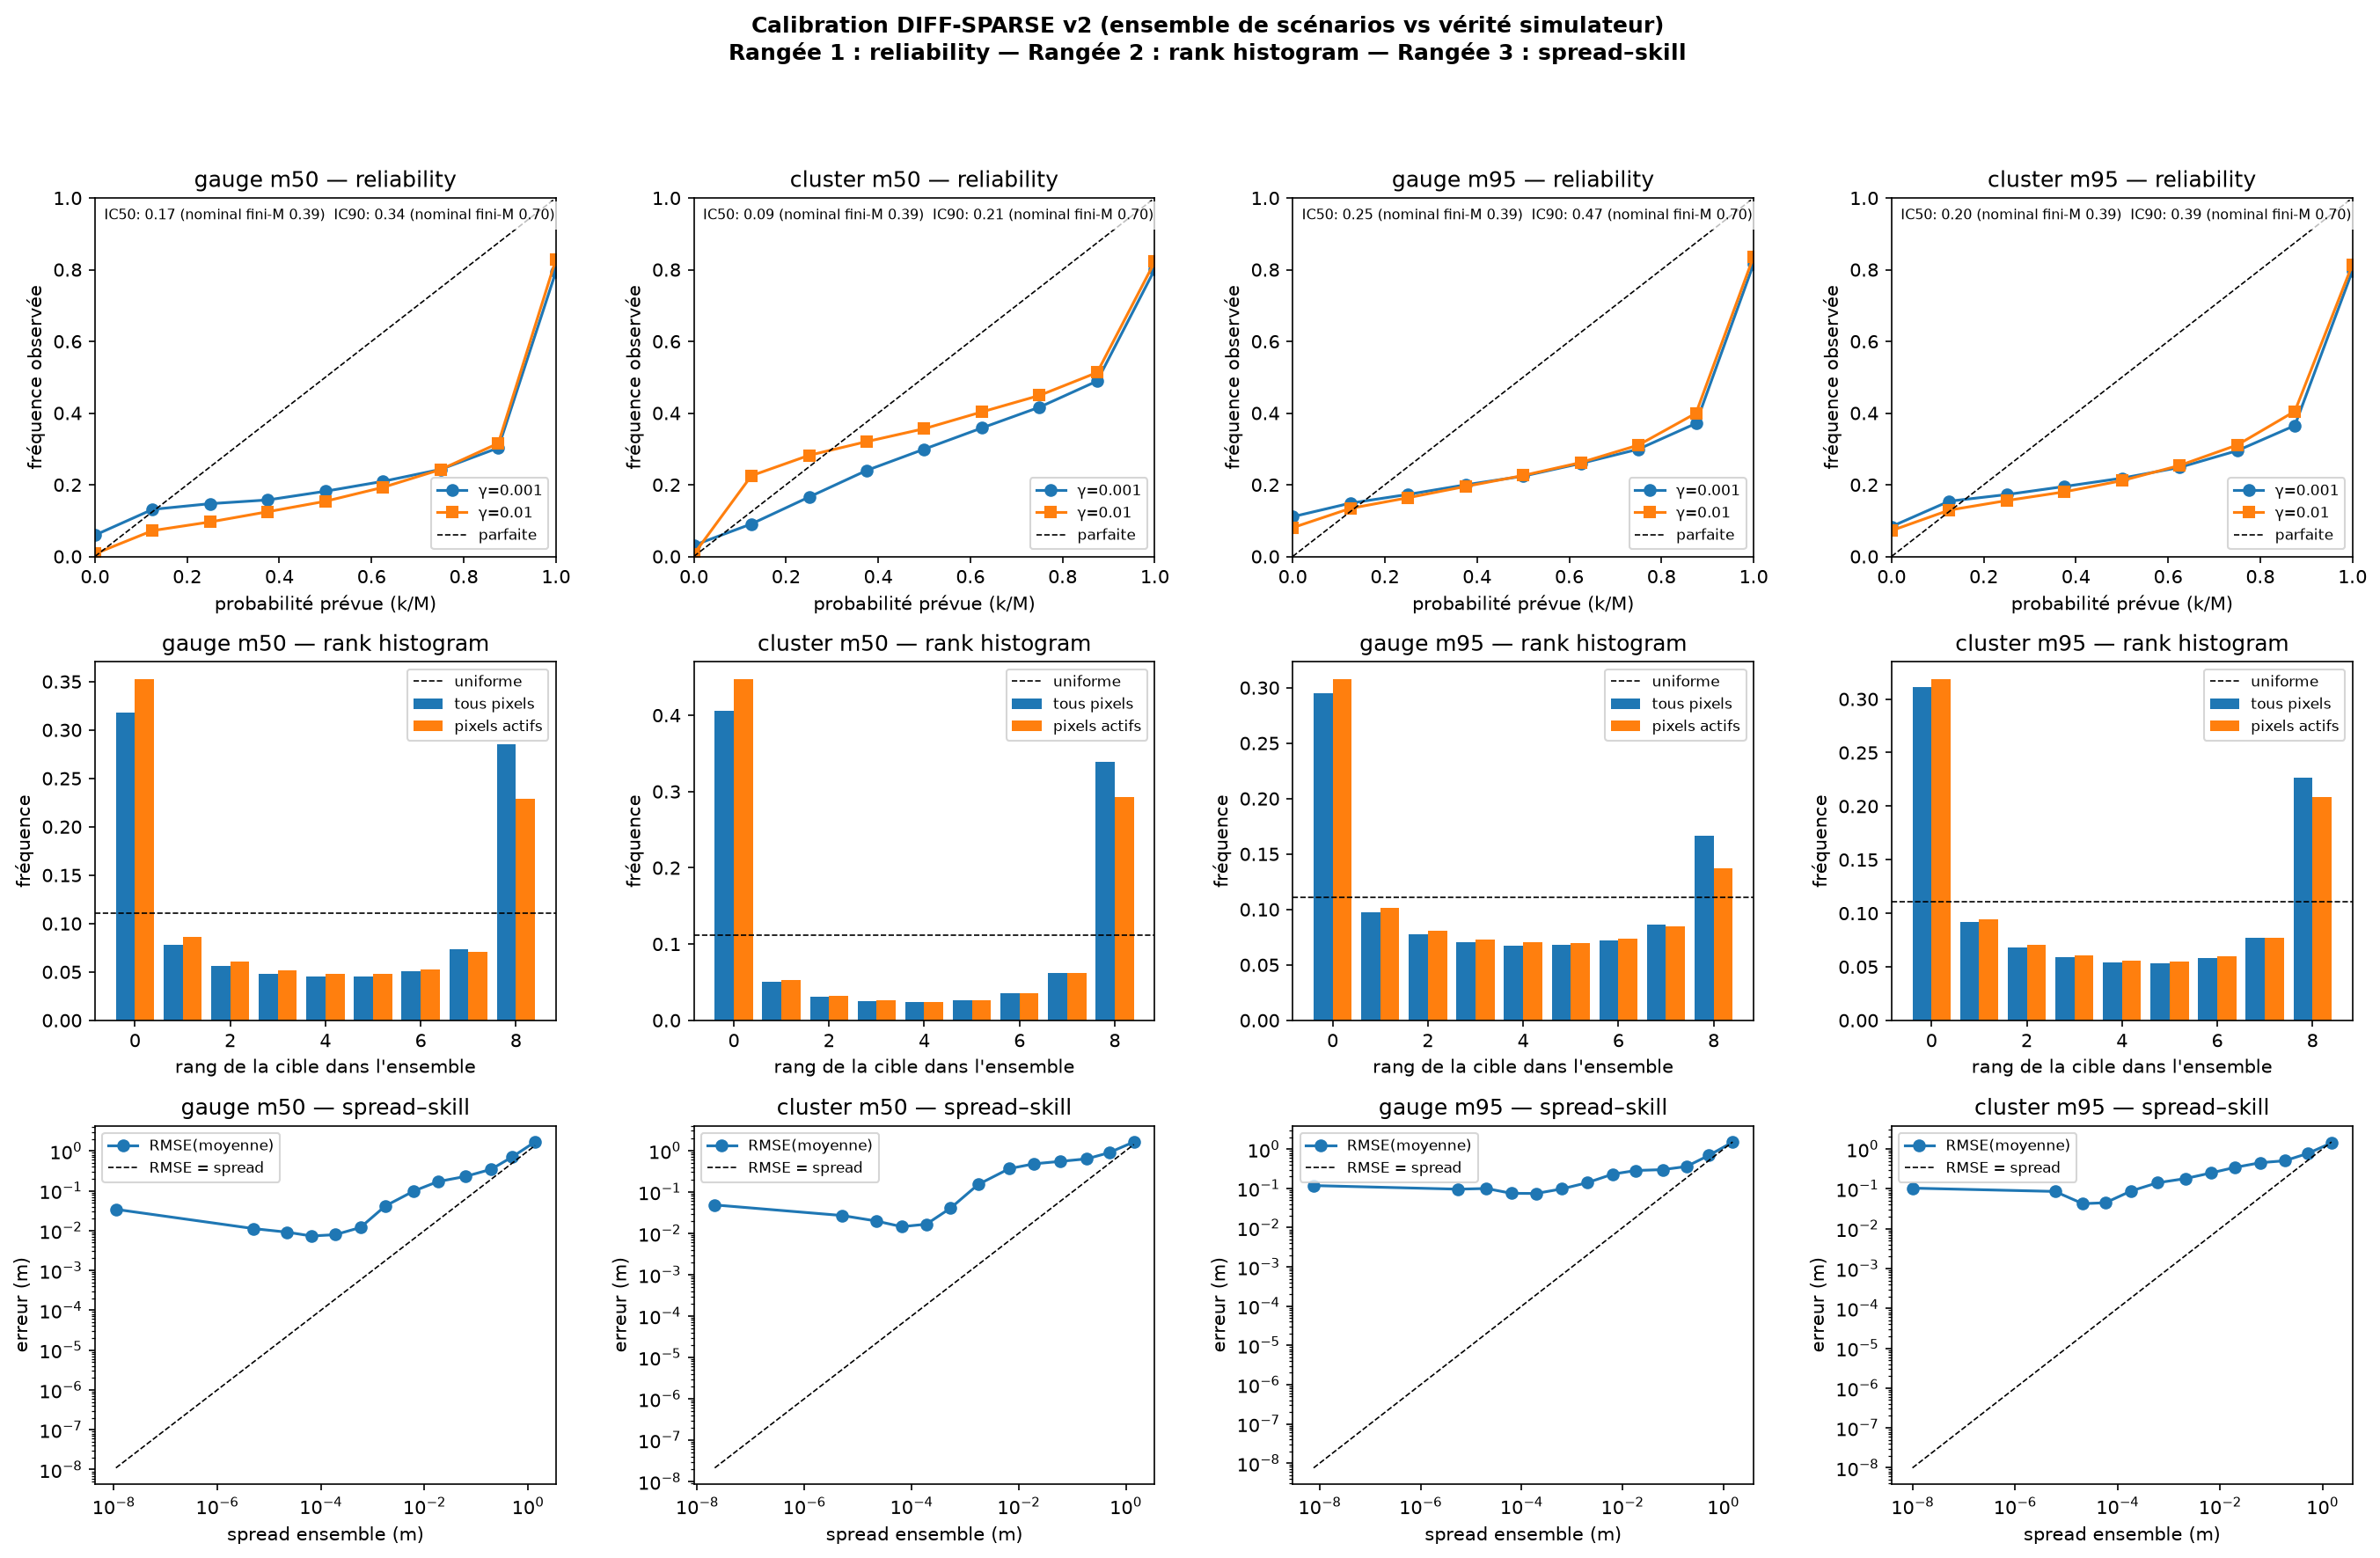
\includegraphics[width=0.92\linewidth]{figures/f5_calibration_wp7.png}
  \caption{Reliability, rank histogram, and spread-skill diagnostics across
  the four structured-mask $\times$ sparsity conditions. Systematic
  under-coverage is visible throughout; sparsity level, not mask structure,
  dominates calibration quality.}
  \label{fig:calibration}
\end{figure}
V2's 8-scenario ensembles show \textbf{severe, systematic under-coverage}
across all tested conditions (Figure~\ref{fig:calibration}): a nominal
90\% central interval (finite-ensemble corrected) covers only 20--47\% of
true outcomes depending on sparsity and mask structure. Sparsity level, not
mask structure, dominates calibration quality (\textsc{m95} is better
calibrated than \textsc{m50} for both mask families, counter-intuitively).

\paragraph{Is a generative model even needed for uncertainty?}
The natural rejoinder --- ``a deterministic model cannot quantify
uncertainty'' --- is false as stated: a \emph{deep ensemble} of
independently trained twins \citep{lakshminarayanan2017deep} is the
standard baseline, and our three twin seeds provide one at zero additional
training cost. Figure~\ref{fig:calibcomp} makes the comparison at
\textsc{m50} on identical metrics and finite-ensemble corrections. The
result is symmetric and sobering: the twin ensemble ($M{=}3$) covers
46--47\% of its corrected nominal intervals, statistically comparable to
V2 ($M{=}8$, 43--48\% under the closest mask condition) --- \textbf{neither
family provides reliable uncertainty out of the box}, and the rank
histograms show V2's ensembles are, if anything, more overconfident in
shape than the twin ensemble's. On this benchmark, calibration as measured
so far does not provide the generative model's missing justification.

\begin{figure}[t]
  \centering
  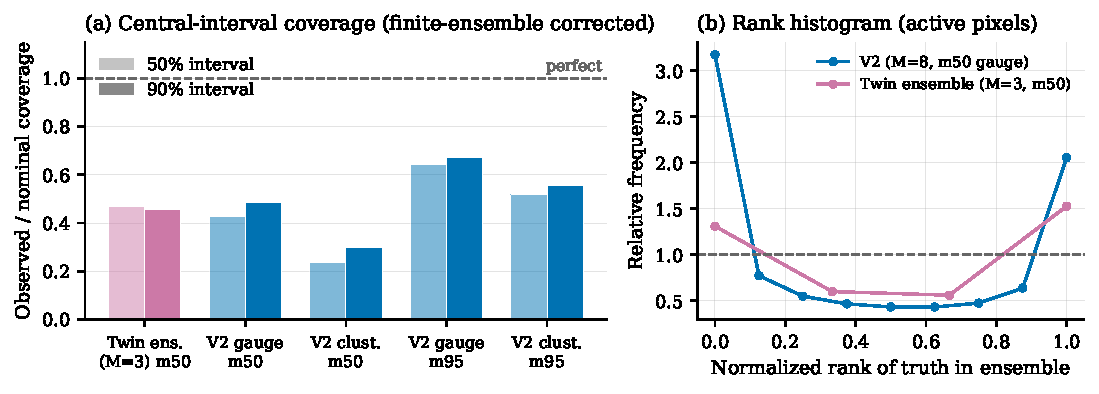
\includegraphics[width=\linewidth]{figures/f6_calibration_comparison.pdf}
  \caption{Uncertainty quality, V2 diffusion ensembles vs.\ a deep ensemble
  of deterministic twins. (a) Observed over nominal coverage
  (finite-ensemble corrected; 1.0 = perfectly calibrated) --- every
  condition is severely under-covered, twin ensemble and V2 alike.
  (b) Rank histograms over active pixels: both are U-shaped
  (overconfident), V2 more strongly so. Caveats: the twin ensemble uses
  random masks at \textsc{m50} while the nearest available V2 evaluations
  use structured masks (the gauge mask is behaviorally closest to random,
  \S\ref{sec:masks}); member counts differ ($M{=}3$ vs $M{=}8$); single-seed
  V2 evaluations. A fully matched comparison (random masks, all sparsities,
  corrected checkpoints) is pending.}
  \label{fig:calibcomp}
\end{figure}

\blocked{Remaining for this subsection: the \textsc{m95} twin-ensemble
evaluation (waiting on the corrected \textsc{m95} twin checkpoints), the
matched random-mask V2 evaluation, and CRPS as a sharpness-aware score to
complement pure coverage.}

\subsection{Ablations, cost, and generalization}
\label{sec:ablations}
\blocked{Table T3 (V2 ablation grid: delta parametrization, target
rainfall, spatial encoder, change-weighted loss, pushforward, diffusion
steps) --- not yet run. Table T4 (Manning roughness from LULC) --- not yet
run. Table T5 (parameter count, inference latency, peak memory, training
wall-clock --- V2 uses 40 diffusion steps $\times$ 8 scenarios per
prediction against the twin's single forward pass; any V2 advantage must be
priced) --- not yet run, cheap (measurement only). Cross-event transfer
(zero-shot evaluation of Australia-trained checkpoints on UK, WP10) and a
second full training/evaluation pass on UK (WP8) --- not yet run.}

% ============================================================
\section{Discussion}
\label{sec:discussion}
\blocked{Written once \S\ref{sec:twinresults} and \S\ref{sec:calibration}'s
WP9 addendum are final. Structural notes: answer the title question
directly and without hedging past what the data supports; state plainly
which regimes (if any) favor the generative model; discuss the
non-monotone dense/\textsc{m50}/\textsc{m95} pattern and what it implies
mechanistically; deployment implications of the cluster-mask degradation;
explicitly discuss the priced cost of any remaining generative advantage
(\S\ref{sec:ablations}).}

\subsection{Limitations}
\label{sec:limitations}
\begin{itemize}
  \item Ground truth is a single deterministic hydraulic simulation per
    event (\S\ref{sec:setup}) --- calibration claims are scoped to
    reconstruction ambiguity, not physical aleatoric uncertainty.
  \item Sparsity is synthetic (random and two structured mask families);
    \blocked{state whatever WP10's zero-shot transfer / real-sensor-layout results show, once available.}
  \item \blocked{Number of events evaluated, once WP8/WP10 are in: currently 1 (Australia), targeting 2 (+ UK).}
\end{itemize}

% ============================================================
\section*{Reproducibility Statement}
Code, configs, and seeds for every reported run are versioned in git.
All headline comparisons use $\geq 3$ seeds; no single-seed number is
reported without an explicit label ruling out generalization. Every model
comparison holds context length and evaluation protocol fixed, with any
remaining asymmetry stated next to the number. Every sparsity regime is
smoke-tested before a training queue is launched --- a discipline adopted
after a live incident (an unguarded scale term produced NaN batches under
the sparse regime specifically, caught and fixed same-day). The
statistical bias specific to deterministic-vs-generative comparisons
(\S\ref{sec:twin}) is documented as a permanent methodological rule after
being caught live on this project's own internal metrics.
\blocked{Repository URL at freeze time.}

% ============================================================
\bibliographystyle{plainnat}
\bibliography{refs}

\end{document}
